\DiaryEntry{First Order Differential Equations (II)}{2018-05-15}{ODE}

\subsubsection{In-homogenuous ODEs}

The solution to the generic in-homogeneous ODE

\bee
y'(t) - a(t)y(t) = g(t), \quad y(0) = y_0
\eee

is given by

\bee
y(t) = y_0 \exp \left( \int_0^t a(s) ds \right) + \int_0^t g(s) \left( \exp \int_s^t a(r)dr \right) ds
\eee

The first integral is the solution to the homogeneous ODE $y'(t) - a(t)y(t) = 0$ (see also last integral in the previous post). The second integral considers the effect of the RHS $g(t)$: Like an initial condition, $g(t)$ is multiplied with $\exp \int_s^t a(r)dr$; but $g(t)$ acts "longer" on the solution, therefore we integrate over all contributions over time (up to $t$).

\paragraph{Constant Input.} We start with the most simple example

\bee
y'(t) - a y(t) = g, \quad y(0) = y_0
\eee

Inserting this into the solution, we obtain

\begin{align*}
y(t) & = y_0 \exp (at) + \int_{s=0}^t g \exp \left[ a(t-s)\right] ds \\
&= y_0 \exp(at) +gexp(at) \int_{s=0}^t g \exp \left[ -as \right] ds \\
&= e^{at} (y_0 + g/a) - g/a
\end{align*}

From this we see that the constant input contributes in two ways to $y(t)$: (i) It acts like an (additional) initial value and correspondingly follows $e^{at}$, and (ii), affects the steady state $\lim_{t \rightarrow \infty} y(t)$, after all transients have decayed. We can see the latter effect by assuming a constant $y(t)$, therefore $y' = 0$: We have $-ay(t) = g \rightarrow y(t) = -g/a$. Assuming $a < 0$ (otherwise there is no steady solution!), $y(t) = g/a$ for $t \rightarrow \infty$. The constant $a$ can be interpreted as "damping factor"; the larger $a$ is, the smaller the contribution from $g(t)$.

The following Figure shows the solution $y(t)$ for $a=-1, g=0$ and initial condition $y_0 = 1$.

\begin{figure}[H]
	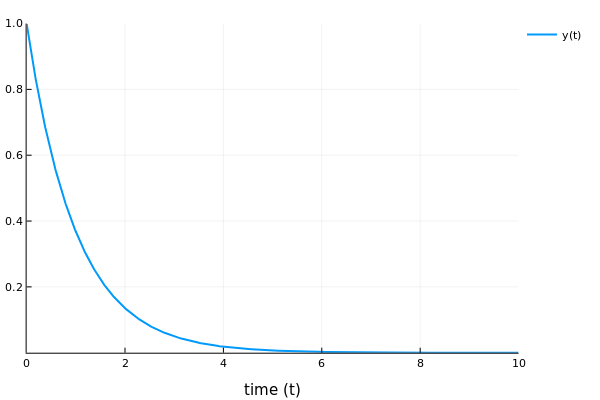
\includegraphics[scale=0.5]{images/ode_02_01.png}
\end{figure}

As a contrast, we plot $y(t)$ with $g=1$ and initial condition $y_0 = 0$ and two different values $a$.

\begin{figure}[H]
	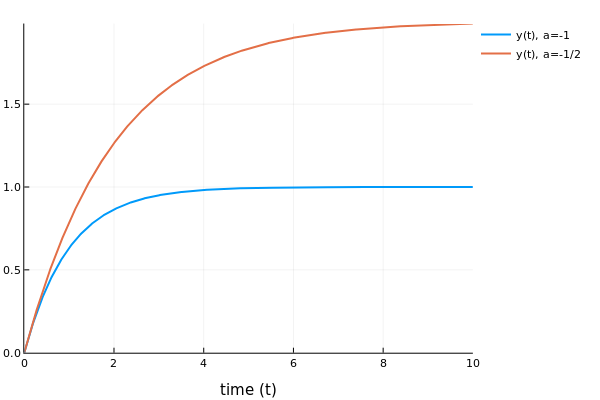
\includegraphics[scale=0.5]{images/ode_02_02.png}
\end{figure}

The effect of $g$ on the steady state of $y(t)$ can be seen and also the effect of $a$ on the time till the steady state is reached.


\paragraph{Sinus Input.} We next consider a sinusoidal input function,

\bee
y'(t) - ay(t) = \sin(t)
\eee

The solution from above yields

\begin{align*}
y(t) &= y_0 \exp \left( \int_0^t a ds \right) + \int_0^t \sin(s) \left( \exp \int_s^t a dr \right) ds = y_0 \exp \left( at \right) + \int_0^t \sin(s) \exp \left( a(t-s) \right) ds \\
&= y_0 \exp \left( at \right) + \exp(at) \int_0^t \sin(s) \exp (-as) ds
\end{align*}

The integral can be calculated analytically and the whole expression can be simplified to

\bee
y(t) = y_0 \exp \left( at \right) - \frac{a \sin(t)+\cos(t) - e^{a t}}{a^2+1} =  \frac{\left[ y_0(a^2+1) + 1 \right] e^{a t} - a \sin(t)-  \cos(t) }{a^2+1}
\eee

We again see two solution parts: An effect of the initial conditions (which decay for $a < 0$) and a steady-state solution which is controlled by $g(t)$. As in the previous example, the factor $a$ controls how strongly $y(t)$ is affected by $g(t)$ - in addition to before (since $g(t)$ is time-varying), $a$ also affects the phase between $g(t)$ and $y(t)$.


The following Figure shows $y(t)$ for two values of $a$ and $y_0=0$ together with $g(t)$. The effect of $a$ on both the amplitude of $y(t)$ and the phase can be clearly seen.

\begin{figure}[H]
	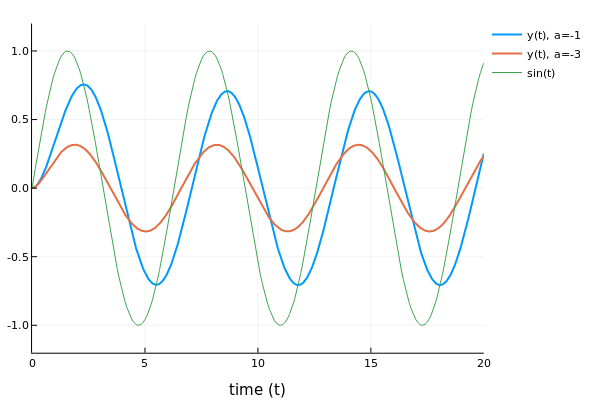
\includegraphics[scale=0.5]{images/ode_02_03.png}
\end{figure}

The next Figure shows the effect of the initial value condition for $y_0 = 2$ and two values of $a$. The parameter controls how fast the initial disturbance of the initial condition  dies off (in addition to the damping/phase shift effects already discussed above).

\begin{figure}[H]
	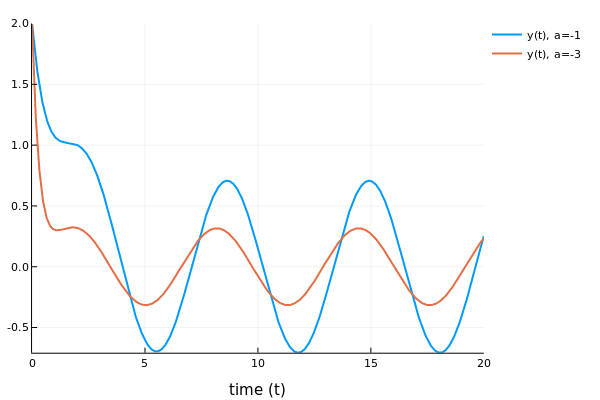
\includegraphics[scale=0.5]{images/ode_02_04.png}
\end{figure}

A solution by Maxima can be obtained as follows

\begin{verbatim}
(%i19)	de:'diff(u,t)-a*u-sin(t);
(de)	'diff(u,t,1)-a*u-sin(t)
(%i20)	gsoln:ode2(de,u,t);
(gsoln)	u=%e^(a*t)*((%e^(-a*t)*(-a*sin(t)-cos(t)))/(a^2+1)+%c)
(%i27)	ic1(gsoln, t=0, u=y0), ratsimp;
(%o27)	u=((a^2+1)*%e^(a*t)*y0-a*sin(t)-cos(t)+%e^(a*t))/(a^2+1)
\end{verbatim}



\paragraph{Sinus Input with varying frequency.} We can extend the previous example to

\bee
y'(t) - ay(t) = \sin(\omega t)
\eee

It is possible to solve this ODE with the same method as the one above; however, the process is rather tedious. Maxima to the rescue yields

\begin{verbatim}
(%i6)	de:'diff(u,t)-a*u-sin(w*t);
gsoln:ode2(de,u,t);
ic1(gsoln, t=0, u=y0), ratsimp;
(de)	-sin(t*w)+'diff(u,t,1)-a*u
(gsoln)	u=%e^(a*t)*((%e^(-a*t)*(-a*sin(t*w)-w*cos(t*w)))/(w^2+a^2)+%c)
(%o6)	u=((%e^(a*t)*w^2+a^2*%e^(a*t))*y0-a*sin(t*w)-w*cos(t*w)+%e^(a*t)*w)/(w^2+a^2)
\end{verbatim}

The solution can be written in "mathematical" notation as

\bee
u=\frac{\left( {{e}^{a t}}\, {{w}^{2}}+{{a}^{2}}\, {{e}^{a t}}\right) \, y_0-a \sin{\left( t w\right) }-w \cos{\left( t w\right) }+{{e}^{a t}} w}{{{w}^{2}}+{{a}^{2}}}
\eee

Besides the transients, we see that the amplitude of the steady state signal decreases with $a^2 + \omega^2$; i.e. lower amplitudes for higher damping and higher frequency.


The following Figure shows $y(t)$ for two different frequencies.

\begin{figure}[H]
	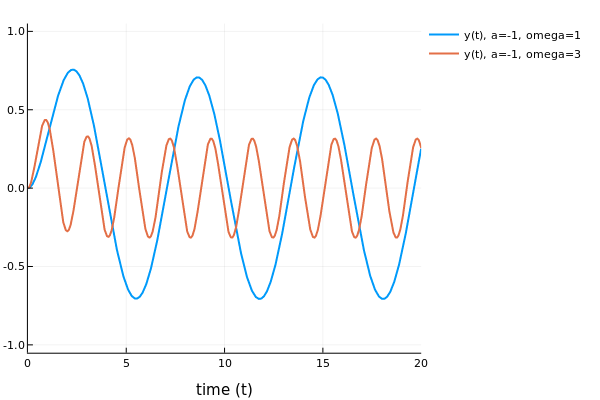
\includegraphics[scale=0.5]{images/ode_02_05.png}
\end{figure}


When we are interested in the steady-state only, we make the following Ansatz for $y(t)$ and use a complex function for $g(t)$:

\bee
y(t) = c \exp(j\omega t)
\eee

Inserting this into the ODE, we obtain

\bee
j c \omega \exp(j\omega t) - a c \exp(j\omega t) = \exp(j\omega t)
\eee

which can be simplified to

\bee
jc \omega - ac = 1 \rightarrow c = \frac{1}{j\omega - a} = \frac{-a-j\omega}{a^2 + \omega^2}
\eee

In order to arrive at a real solution with $g(t) = \sin(\omega t)$, we take the imaginary part of $c \exp(j \omega t)$:

\bee
\Im \left( c \exp(j \omega t) \right) = \Im \left( \frac{-a-j\omega}{a^2 + \omega^2}  \exp(j \omega t) \right) = \frac{-a \sin (\omega t) - \omega \cos (\omega t)}{a^2 + \omega^2}
\eee

Note that this corresponds with the steady-state solution from Maxima.

The following Figure shows the ODE solution and the analytical steady-state solution. After decay of the transients, the steady state of the ODE solution and the analytical one are equal.

\begin{figure}[H]
	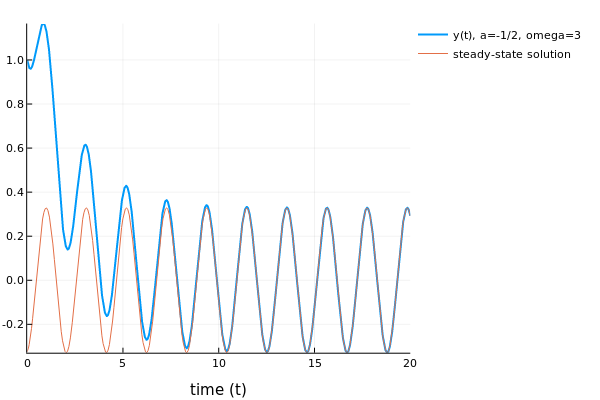
\includegraphics[scale=0.5]{images/ode_02_06.png}
\end{figure}
